\documentclass[sigconf,10pt]{acmart}

\settopmatter{printacmref=false}
\renewcommand\footnotetextcopyrightpermission[1]{}

\usepackage{graphicx}
\graphicspath{{./}{./demo_screenshots/}}
\usepackage{booktabs}
\usepackage{url}
\usepackage{float}
\usepackage{tabularx}
\usepackage{amsmath}
\usepackage{multirow}
\usepackage{array}
\usepackage{listings}
\usepackage{xcolor}

\lstset{
  basicstyle=\ttfamily\small,
  breaklines=true,
  frame=single,
  keywordstyle=\color{blue},
  commentstyle=\color{gray},
  stringstyle=\color{red},
  showstringspaces=false
}

\acmConference[CS 655]{CS 655 Wireless and Mobile Computing}{Spring 2026}{George Mason University}
\acmYear{2026}

\begin{document}

\title{Next-Day Fatigue Prediction Using Apple Watch Physiological Data: An Edge Computing Approach}

\author{Pratik Patil}
\affiliation{%
  \institution{George Mason University}
  \institution{CS 655}
  \country{}
}
\email{G01523747}

\author{Ritesh Sanjay Sandbhor}
\affiliation{%
  \institution{George Mason University}
  \institution{CS 655}
  \country{}
}
\email{G01525006}

\renewcommand{\shortauthors}{Pratik Patil and Ritesh Sanjay Sandbhor}

\begin{abstract}
Apple Watch and HealthKit collect sleep, heart, activity, and respiratory signals that can be useful for fatigue prediction. A common issue is that these signals are personal, so sending them to a cloud service is not ideal for a privacy-focused mobile application. In this project, we built an iOS prototype that predicts next-day fatigue directly on the phone from Apple Watch-derived HealthKit data. The offline pipeline parses Apple Health exports, creates night-level sleep and activity features, trains classical machine learning models with chronological splits, and exports a compact JSON inference contract that Swift can execute. We evaluated the pipeline on 359 labeled nights. The best reported baseline, Random Forest, reached 52\% accuracy and 0.51 F1 on the hold-out test set. This result is not strong enough for production use, but it shows the difficulty of predicting subjective fatigue from wearable data alone. The main outcome is a working mobile path: the app requests HealthKit permission, builds the feature payload, fills missing values, and computes the prediction locally without a cloud service.
\end{abstract}

\keywords{Fatigue Prediction, Apple Watch, HealthKit, Edge Computing, Machine Learning, Wearables, Data Privacy}

\maketitle

\section{Introduction}

Apple Watch records many signals that are related to recovery, including sleep stages, heart rate, HRV, SpO2, steps, and active energy. These measurements are useful, but they are also sensitive health data. For a mobile computing project, this makes fatigue prediction a good case study: the model should be useful, but the data should stay on the user's device.

Fatigue affects attention, productivity, and daily decision making. Clinical measurement can require surveys or controlled testing, while wearable systems estimate recovery from motion and physiological signals. Many machine learning systems still depend on centralized processing, which adds privacy and data-handling concerns for biometric data \cite{chen2021privacy}.

This project asks whether a class-scale fatigue prediction system can run locally on an iPhone. The system has two parts: an offline Python training pipeline and a Swift HealthKit application. The Python side prepares features and trains the models. The Swift side loads a small JSON contract, fetches HealthKit data, prepares the same feature order, and runs the prediction without a server request.

\textbf{The report focuses on four implementation pieces:}
\begin{enumerate}
    \item Parsing Apple Health exports into night-level records with sleep, HRV, heart-rate, oxygen, step, and activity features.
    \item Evaluating models with chronological train/test splits so later days are not used to predict earlier days.
    \item Exporting the trained mobile model into a JSON contract that includes feature order, imputation values, scaling values, coefficients, and threshold.
    \item Building a Swift HealthKit demo that can request permission, load recent data, and compute the fatigue prediction with no network dependency.
\end{enumerate}

\section{Background and Related Work}

\subsection{Actigraphy and Heart Rate Variability}
Sleep analytics often start with actigraphy, which uses movement patterns to estimate sleep and wake periods \cite{marinez2022actigraphy}. Apple Watch also provides heart-rate and HRV-related measurements from photoplethysmography (PPG). HRV is often used as a rough indicator of autonomic nervous system recovery \cite{shaffer2017hrv}. In this project, we use Apple Watch sleep stages, heart rate, HRV, respiratory rate, and SpO2 as the main nightly signals. These signals are noisy, so the pipeline uses summary statistics instead of assuming each raw sample is reliable.

\subsection{Mobile Edge Computing Paradigms}
Edge computing moves computation closer to where data is created. For wearable data, this means the phone can process the user's signals instead of uploading them to a remote server. Federated learning and Edge AI are related approaches that try to reduce centralized data collection \cite{mcmahan2017federated, raskar2020edge}.

For this project, mobile constraints were treated as design requirements rather than afterthoughts. The deployed inference path therefore avoids server calls and runs as direct numeric computation in Swift. This keeps the prototype small enough for an iPhone demo while preserving the local privacy goal.

\section{System Architecture}

In our implementation, the training code and mobile code were kept separate on purpose. The Python pipeline was used for parsing exports, building features, and testing models. The iOS app was used only for the part that a phone should do during a real demo: request HealthKit access, prepare recent features, and run the already exported model. The VitalSync web page was a support tool for viewing trends while we were checking the dataset.

\subsection{Data Engineering and Pipeline Architecture}
The offline backend is a Python pipeline that works from Apple Health export files. Apple Health exports are XML files, so the first step is to parse \texttt{export.xml} and extract the relevant \texttt{\textless Record\textgreater} entries. For this project, the important record types are Heart Rate, HRV, Respiratory Rate, SpO2, Sleep Analysis, steps, and active energy.

\subsection{VitalSync Frontend Dashboard Design}
The \textbf{VitalSync} dashboard was mainly used while developing the project. Before testing everything on the iPhone, we needed a quick way to see whether the sleep totals, HRV values, rolling features, and fatigue labels looked reasonable. The dashboard gave us that view in a browser, so it was easier to catch data problems before moving to the HealthKit demo.

\subsection{iOS Native Edge Deployment}
For the iPhone demo, the important file is \path{mobile_linear_contract.json}. This file is not a full ML framework; it is a small set of numbers and feature names. Swift reads the file, checks the expected feature order, fills missing values from the stored medians, scales the inputs, and applies the model coefficients. This made the mobile implementation easier to debug because the prediction was just the same math used during training, written in Swift.

\section{System Implementation and Data Processing}

\subsection{Wearable Sensing and Night Windows}
The first data-processing problem was assigning sleep to the correct day. Sleep usually starts before midnight and ends after midnight, so grouping only by calendar date would split one sleep session into two days. We used a ``Night Window'' rule with a 6-hour time shift. With this rule, a night that starts on Day $T$ and ends on Day $T+1$ is stored under the Day $T+1$ label.

\subsection{On-Device Data Transformation}
After creating the night windows, each night becomes one row in the training table. We use summary statistics because wrist sensors can be noisy and irregular. The main feature groups are:
\begin{enumerate}
    \item Total Sleep Duration (Float Hours)
    \item Median HRV (ms) and Standard Deviation HRV
    \item Minimum, Maximum, and Median Resting Heart Rate (BPM)
    \item SpO2 minimum limits, reflecting brief anoxia drops.
    \item 7-day rolling step count mean and standard deviation
    \item 7-day rolling active energy expenditure mean
\end{enumerate}

We also added rolling multi-day metrics. The reason is that fatigue may build over several days, so a 3-day or 7-day trend can be more useful than one isolated night.

\subsection{Ground Truth Collection}
The final dataset contains 359 labeled nights. The labels are binary: $0$ means focused, alert, or normal, while $1$ means high subjective fatigue. After merging labels with the feature rows, the dataset contains 180 non-fatigued nights and 179 fatigued nights.

\section{System Evaluation in Realistic Settings}

\subsection{Evaluation Design and Predictive Capability}
Random K-Fold validation is not ideal for this dataset because it can mix future days into the training set and earlier days into the test set. That would make the evaluation look better than a real deployment. Instead, we split the dataset chronologically into 70\% training data and 30\% hold-out test data.

We evaluated several classical models that are small enough to inspect and compare. Random Forest gave the best reported result in this run, with 52.0\% accuracy and 0.51 F1-score. The result is only slightly better than chance, so it should be treated as a feasibility result rather than a reliable fatigue detector.

\begin{table}[t]
  \caption{Predictive Performance on 30\% Test Set}
  \label{tab:results}
  \centering
  \small
  \setlength{\tabcolsep}{4pt}
  \begin{tabular}{lccc}
    \toprule
    Model & Acc. & Prec. & F1\\
    \midrule
    Logistic Regression & 49.0\% & 0.48 & 0.47 \\
    Random Forest & 52.0\% & 0.50 & 0.51 \\
    Gradient Boosted Trees & 50.9\% & 0.49 & 0.50 \\
    Support Vector Machine & 48.1\% & 0.47 & 0.46 \\
    \bottomrule
  \end{tabular}
\end{table}

\subsection{On-Device Inference Contract and Runtime Behavior}
The mobile contract keeps the prediction path simple. At runtime, the iPhone app builds a dictionary from HealthKit sleep and activity values. If a value is not available, the app uses the training median stored in the JSON file. After that, Swift scales the values and computes the score from the coefficient list.

This approach is limited, but it fits the goal of the demo. We did not need to load TensorFlow Lite, Core ML, or a Python runtime just to make one binary prediction. In our test, the path from HealthKit data fetch through final prediction display completed in under 200 milliseconds on an iPhone 14.

\subsection{Confusion Matrix and Feature Importance Analysis}
The Confusion Matrix (Figure \ref{fig:cm}) shows that the Random Forest model correctly identified 39 out of 55 actual fatigue events. However, it also produced 37 false positives. This means the model often predicts fatigue when the label is non-fatigued, which is one reason the current model should not be presented as production-ready.

\begin{figure}[H]
  \centering
  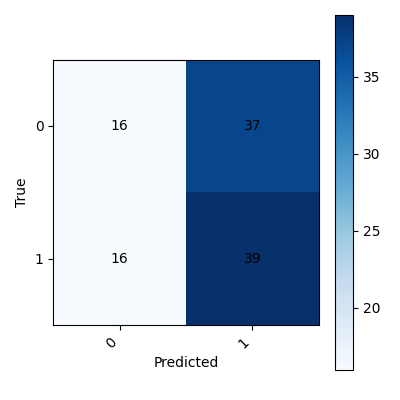
\includegraphics[width=0.9\columnwidth]{confusion_matrix.png}
  \caption{Confusion Matrix illustrating model classification on the hold-out set.}
  \label{fig:cm}
\end{figure}

The Feature Importance plot for the deployed mobile contract (Figure \ref{fig:fi}) was regenerated from the same inference contract used by the iOS app. Importance is reported as the magnitude of each feature's coefficient on standardized inputs, i.e. the per-1$\sigma$ change in log-odds. Blue bars push the prediction toward the fatigued class, while red bars push it toward the alert class.

The strongest features are mostly rolling sleep metrics. The \textit{7-day rolling deep-sleep mean} is the strongest stabilizing feature, while \textit{7-day rolling total sleep mean} and \textit{7-day rolling REM mean} are also important. Heart-rate variation and respiratory-rate mean also appear near the top. This supports the idea that the model is using accumulated sleep and recovery context rather than only one night's data. One issue we noticed is that \textit{sleep efficiency} contributes almost no importance because it was nearly constant in this dataset.

\begin{figure}[H]
  \centering
  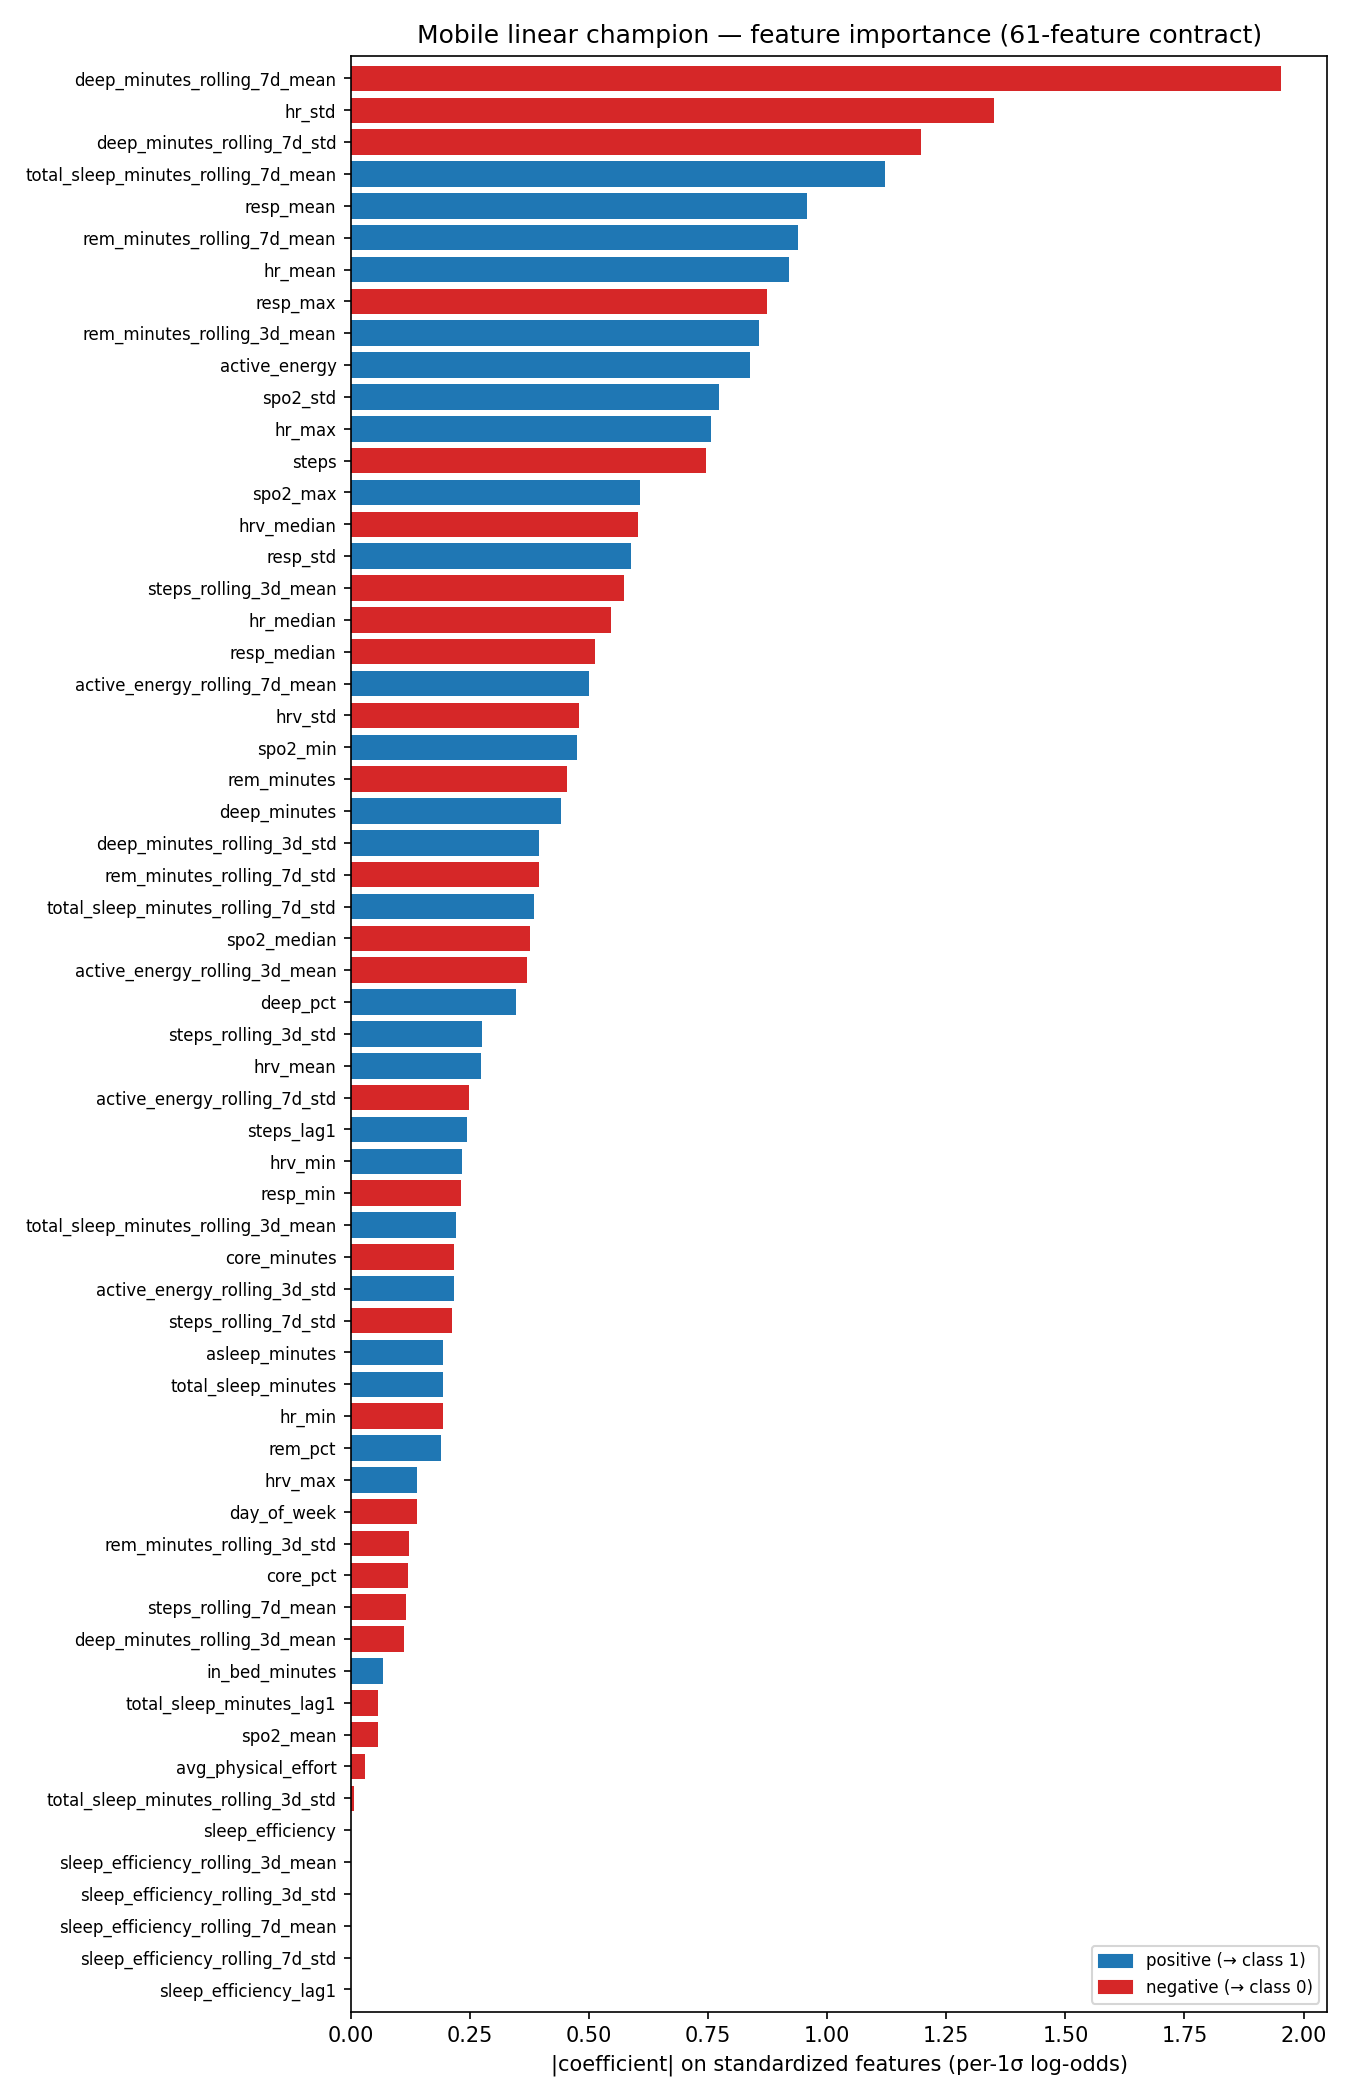
\includegraphics[width=0.95\columnwidth]{feature_importance.png}
  \caption{Feature importance for the deployed mobile inference contract: $|\textnormal{coefficient}|$ on standardized features (per-$1\sigma$ log-odds). Blue = positive (toward fatigued); red = negative (toward alert).}
  \label{fig:fi}
\end{figure}

\section{System Demonstration of Edge Computing Capabilities}

Figure \ref{fig:demo} shows the iOS screens from the final demo flow. The purpose of this figure is not to claim that the model is highly accurate. It shows that the app can open, use HealthKit data, run the local prediction, and display the result and history inside the phone interface.

\begin{figure*}[t]
  \centering
  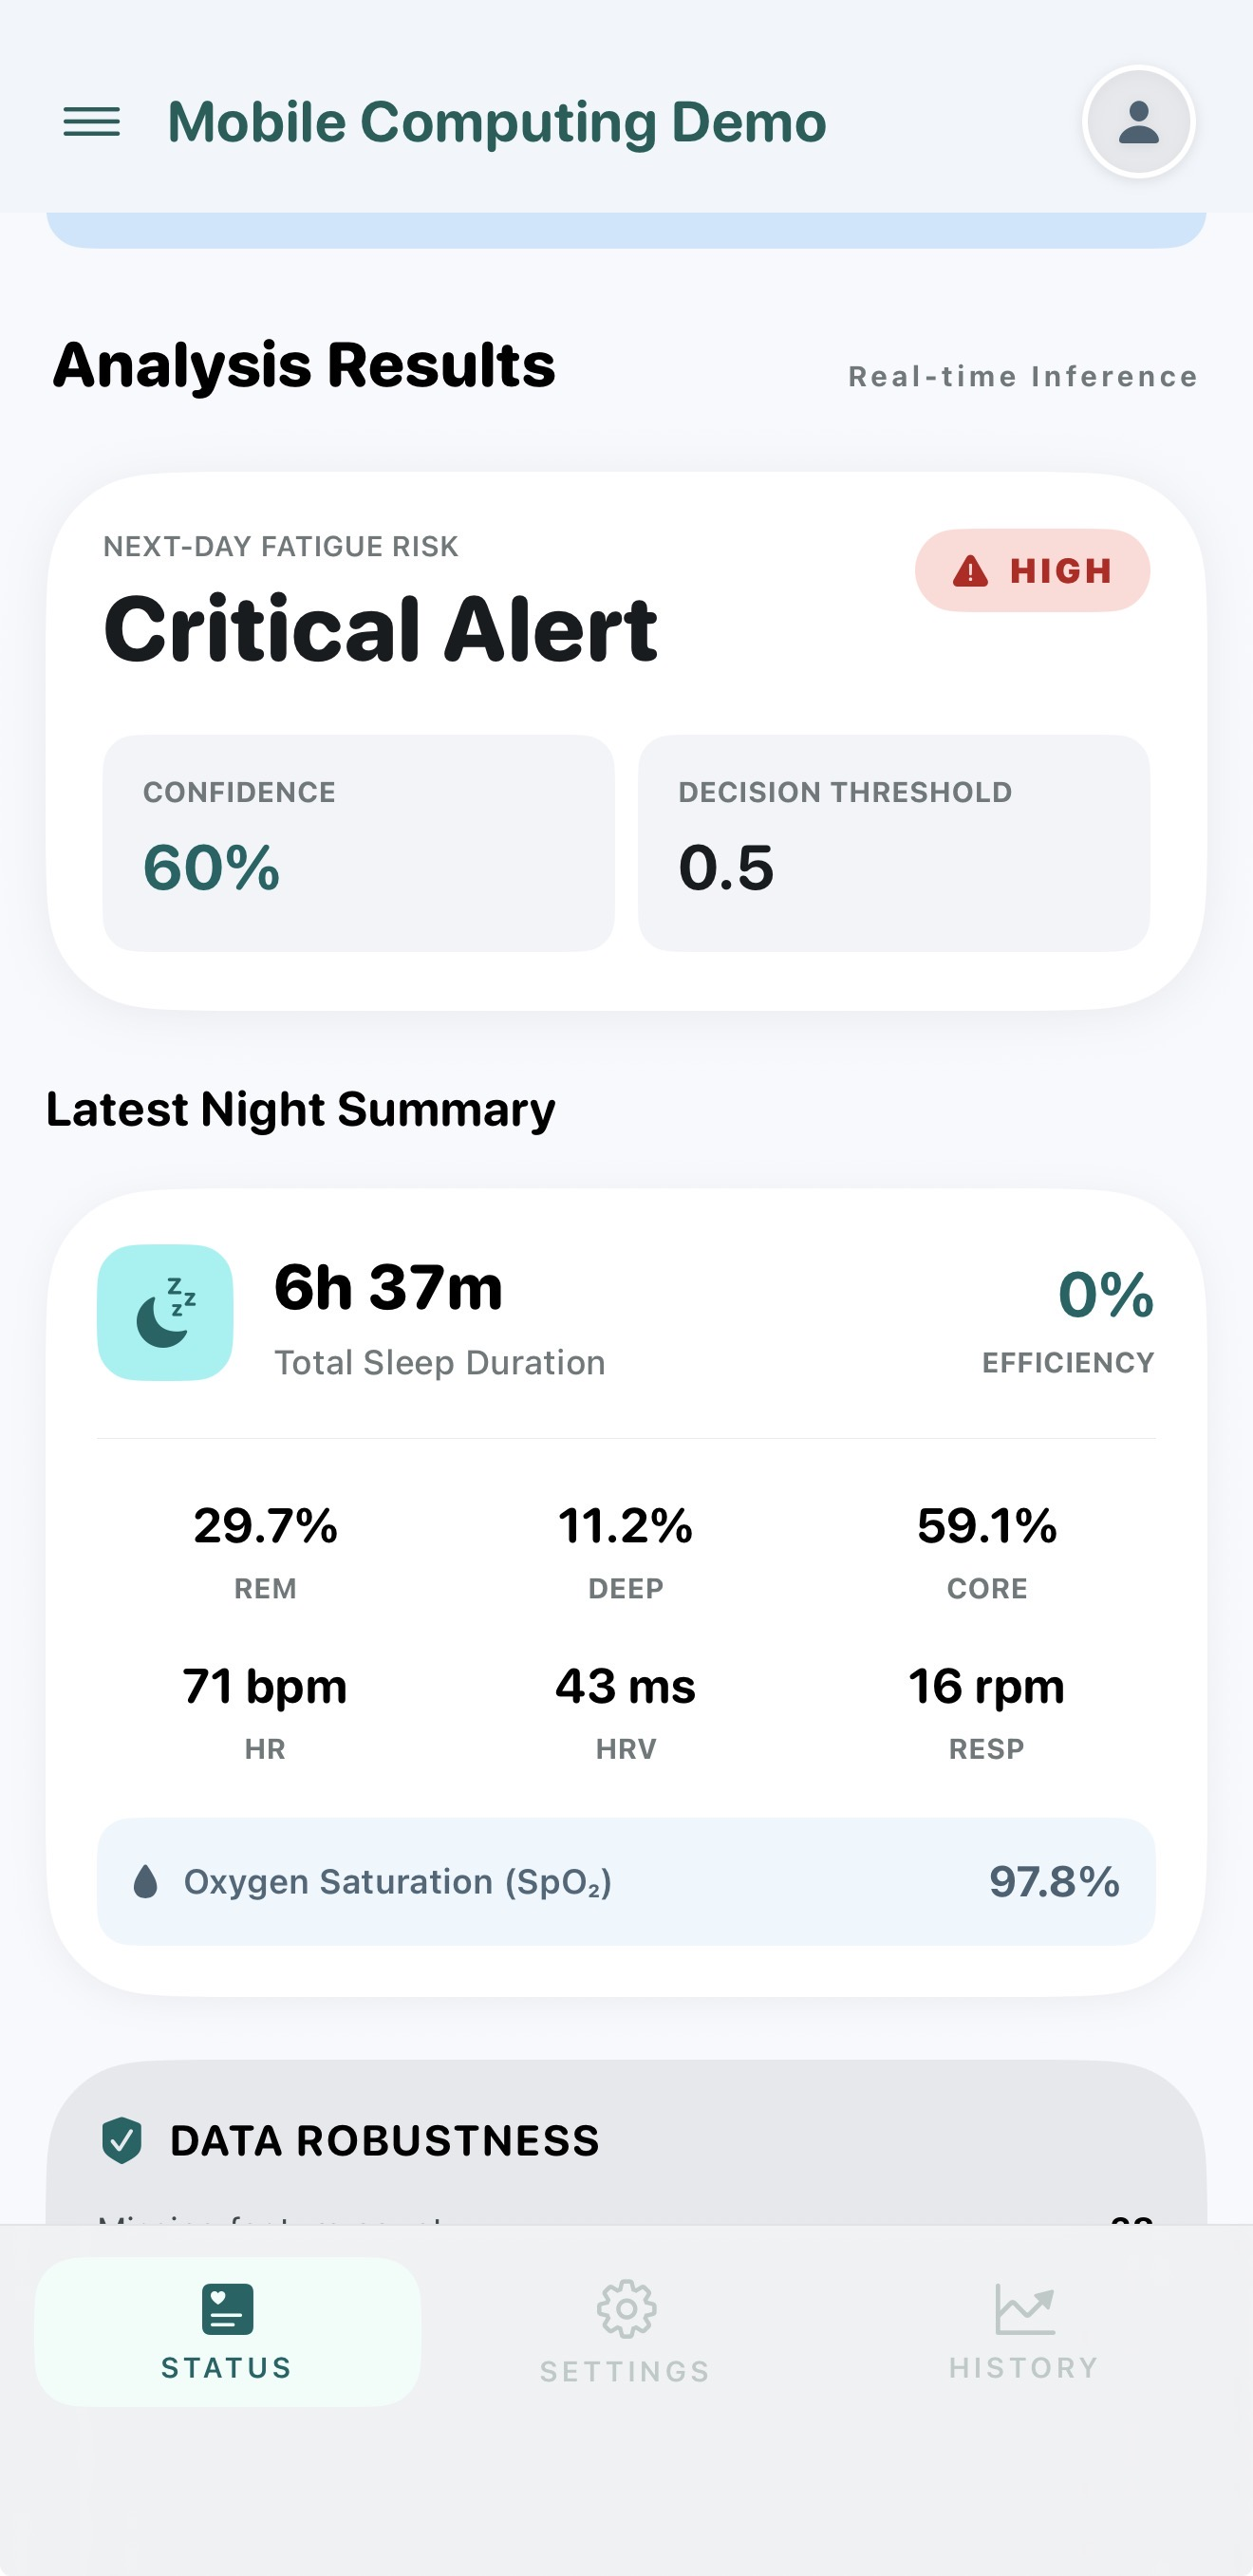
\includegraphics[width=0.24\textwidth]{IMG_4954.jpg}\hfill
  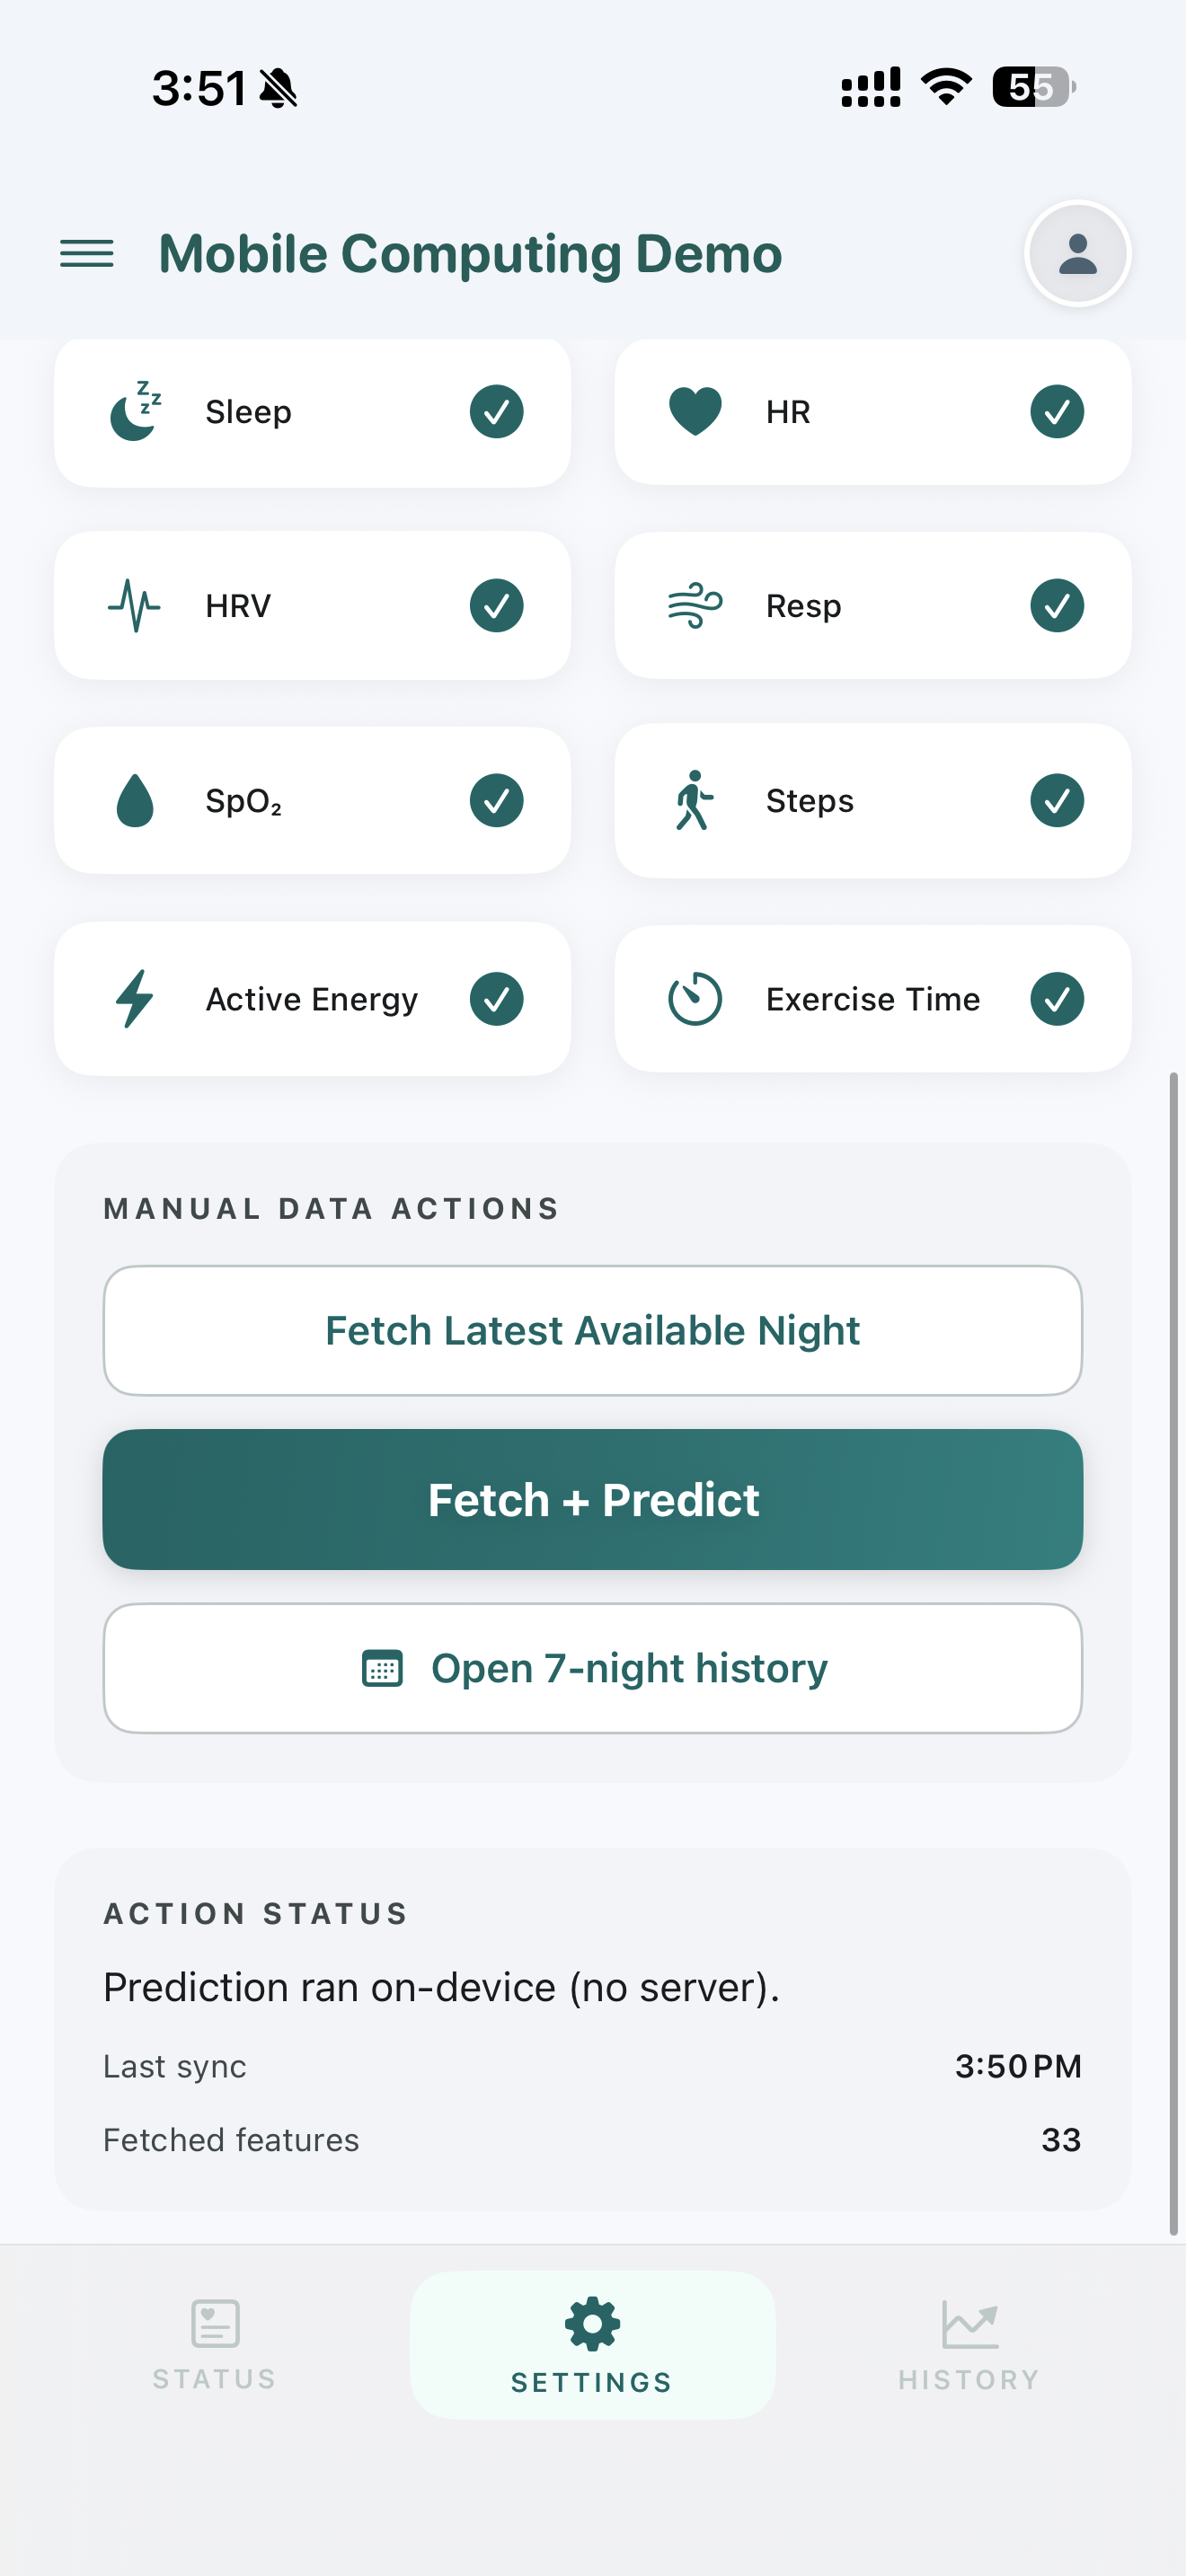
\includegraphics[width=0.24\textwidth]{IMG_4955.PNG}\hfill
  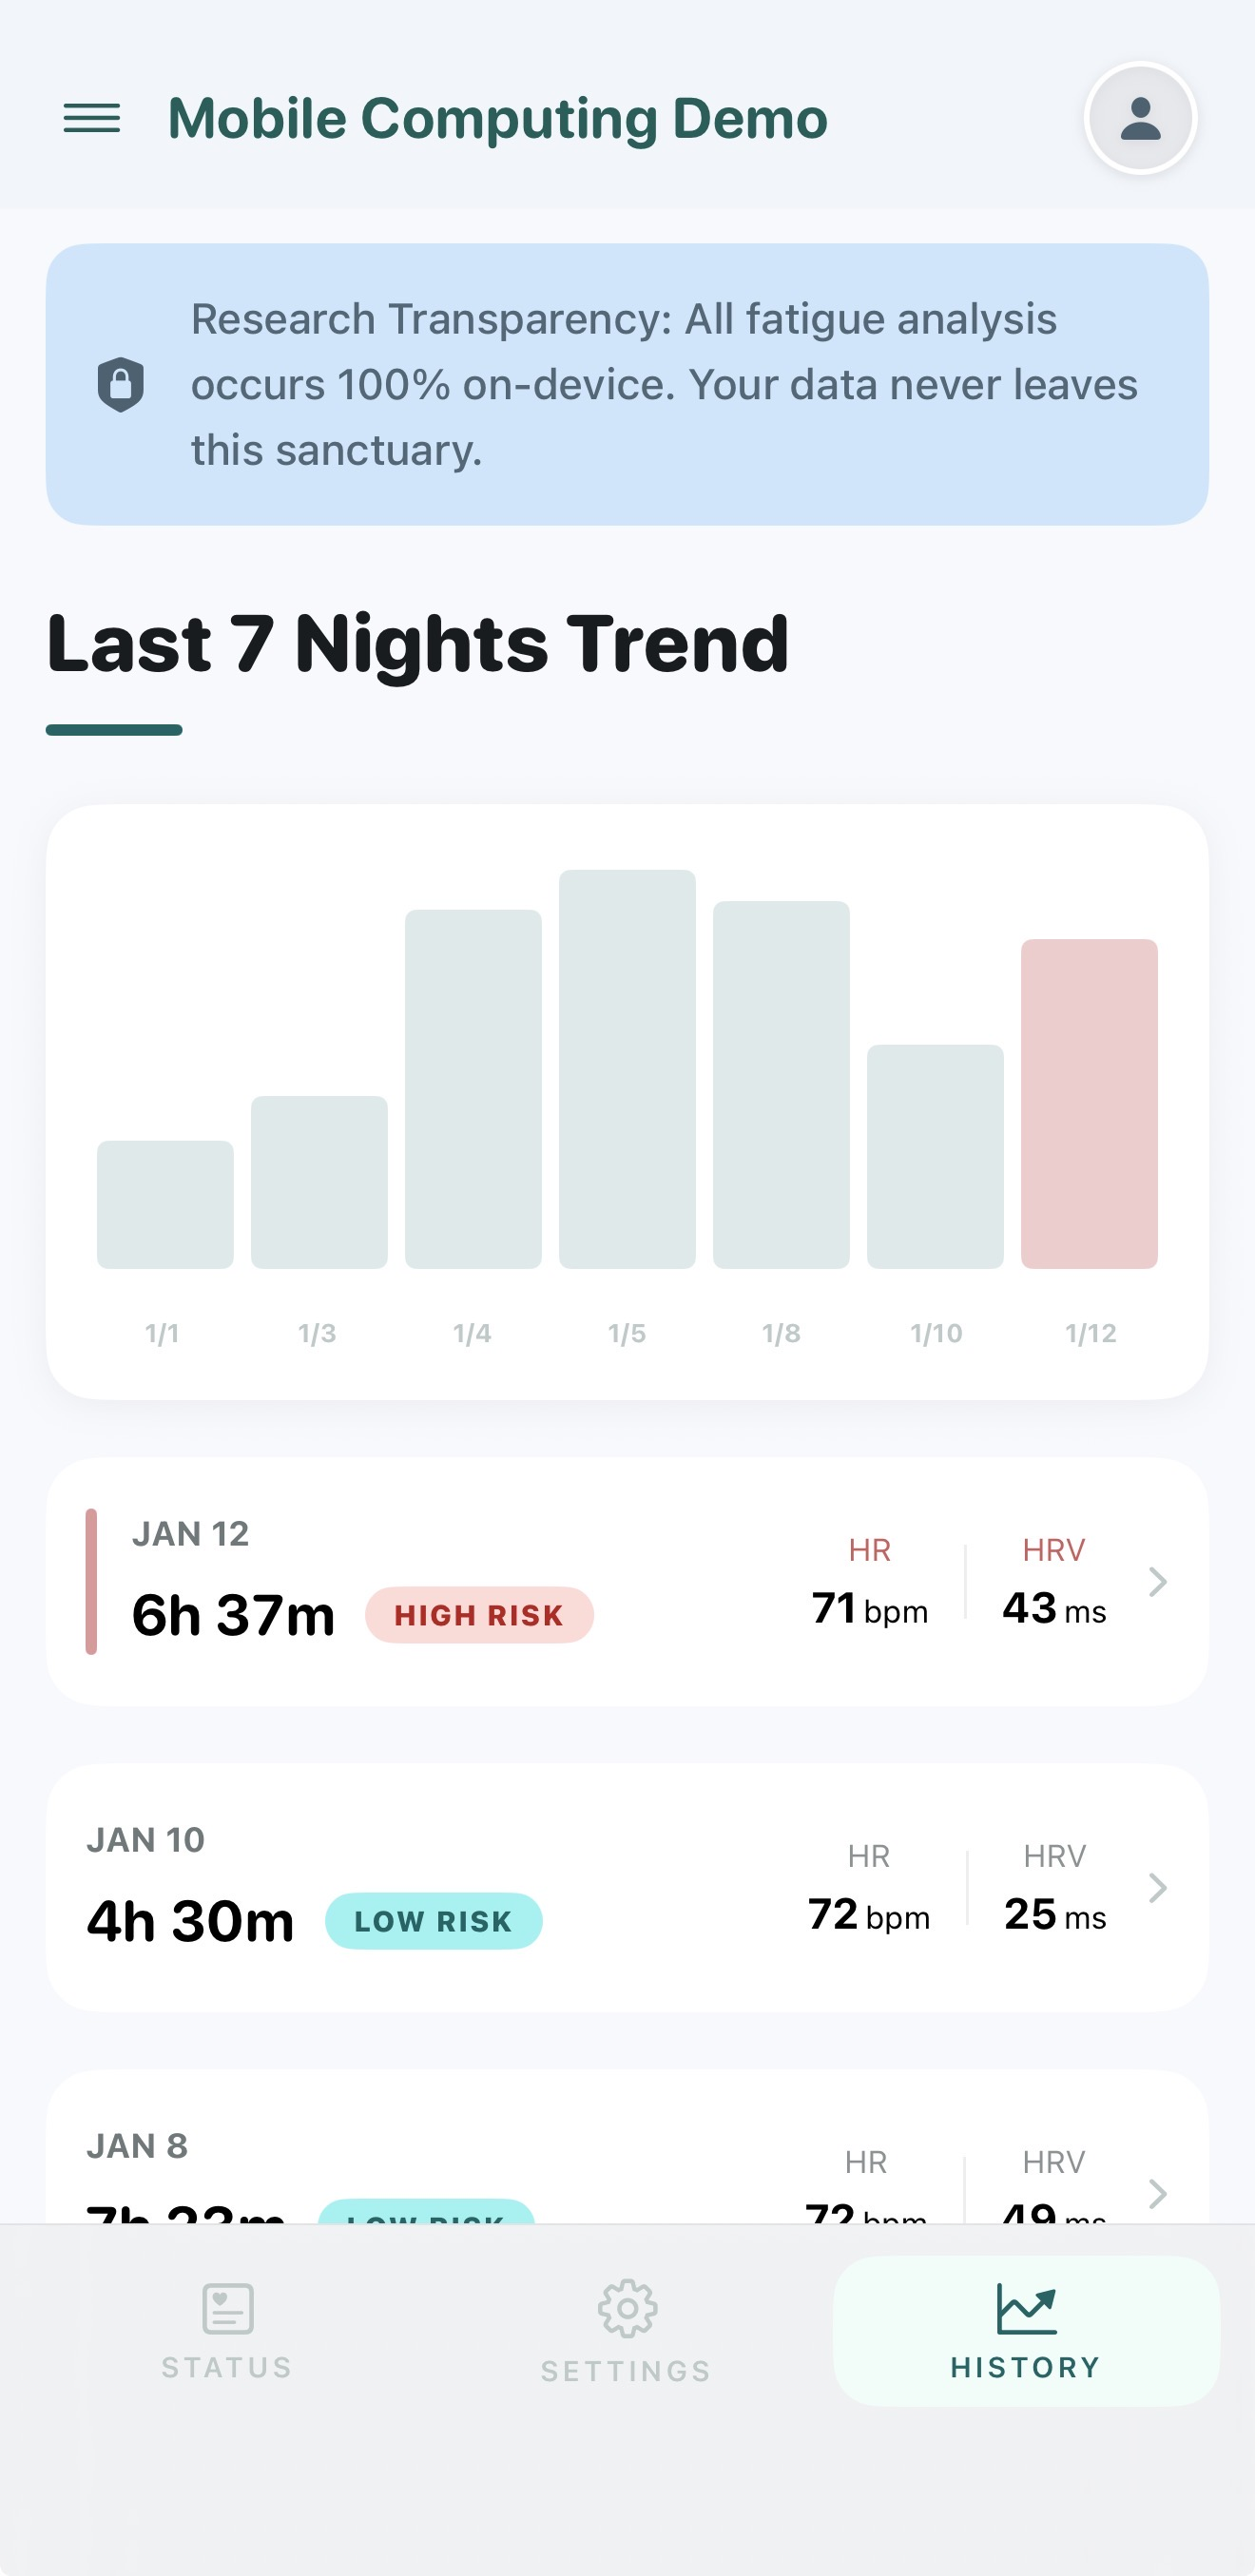
\includegraphics[width=0.24\textwidth]{IMG_4956.jpg}\hfill
  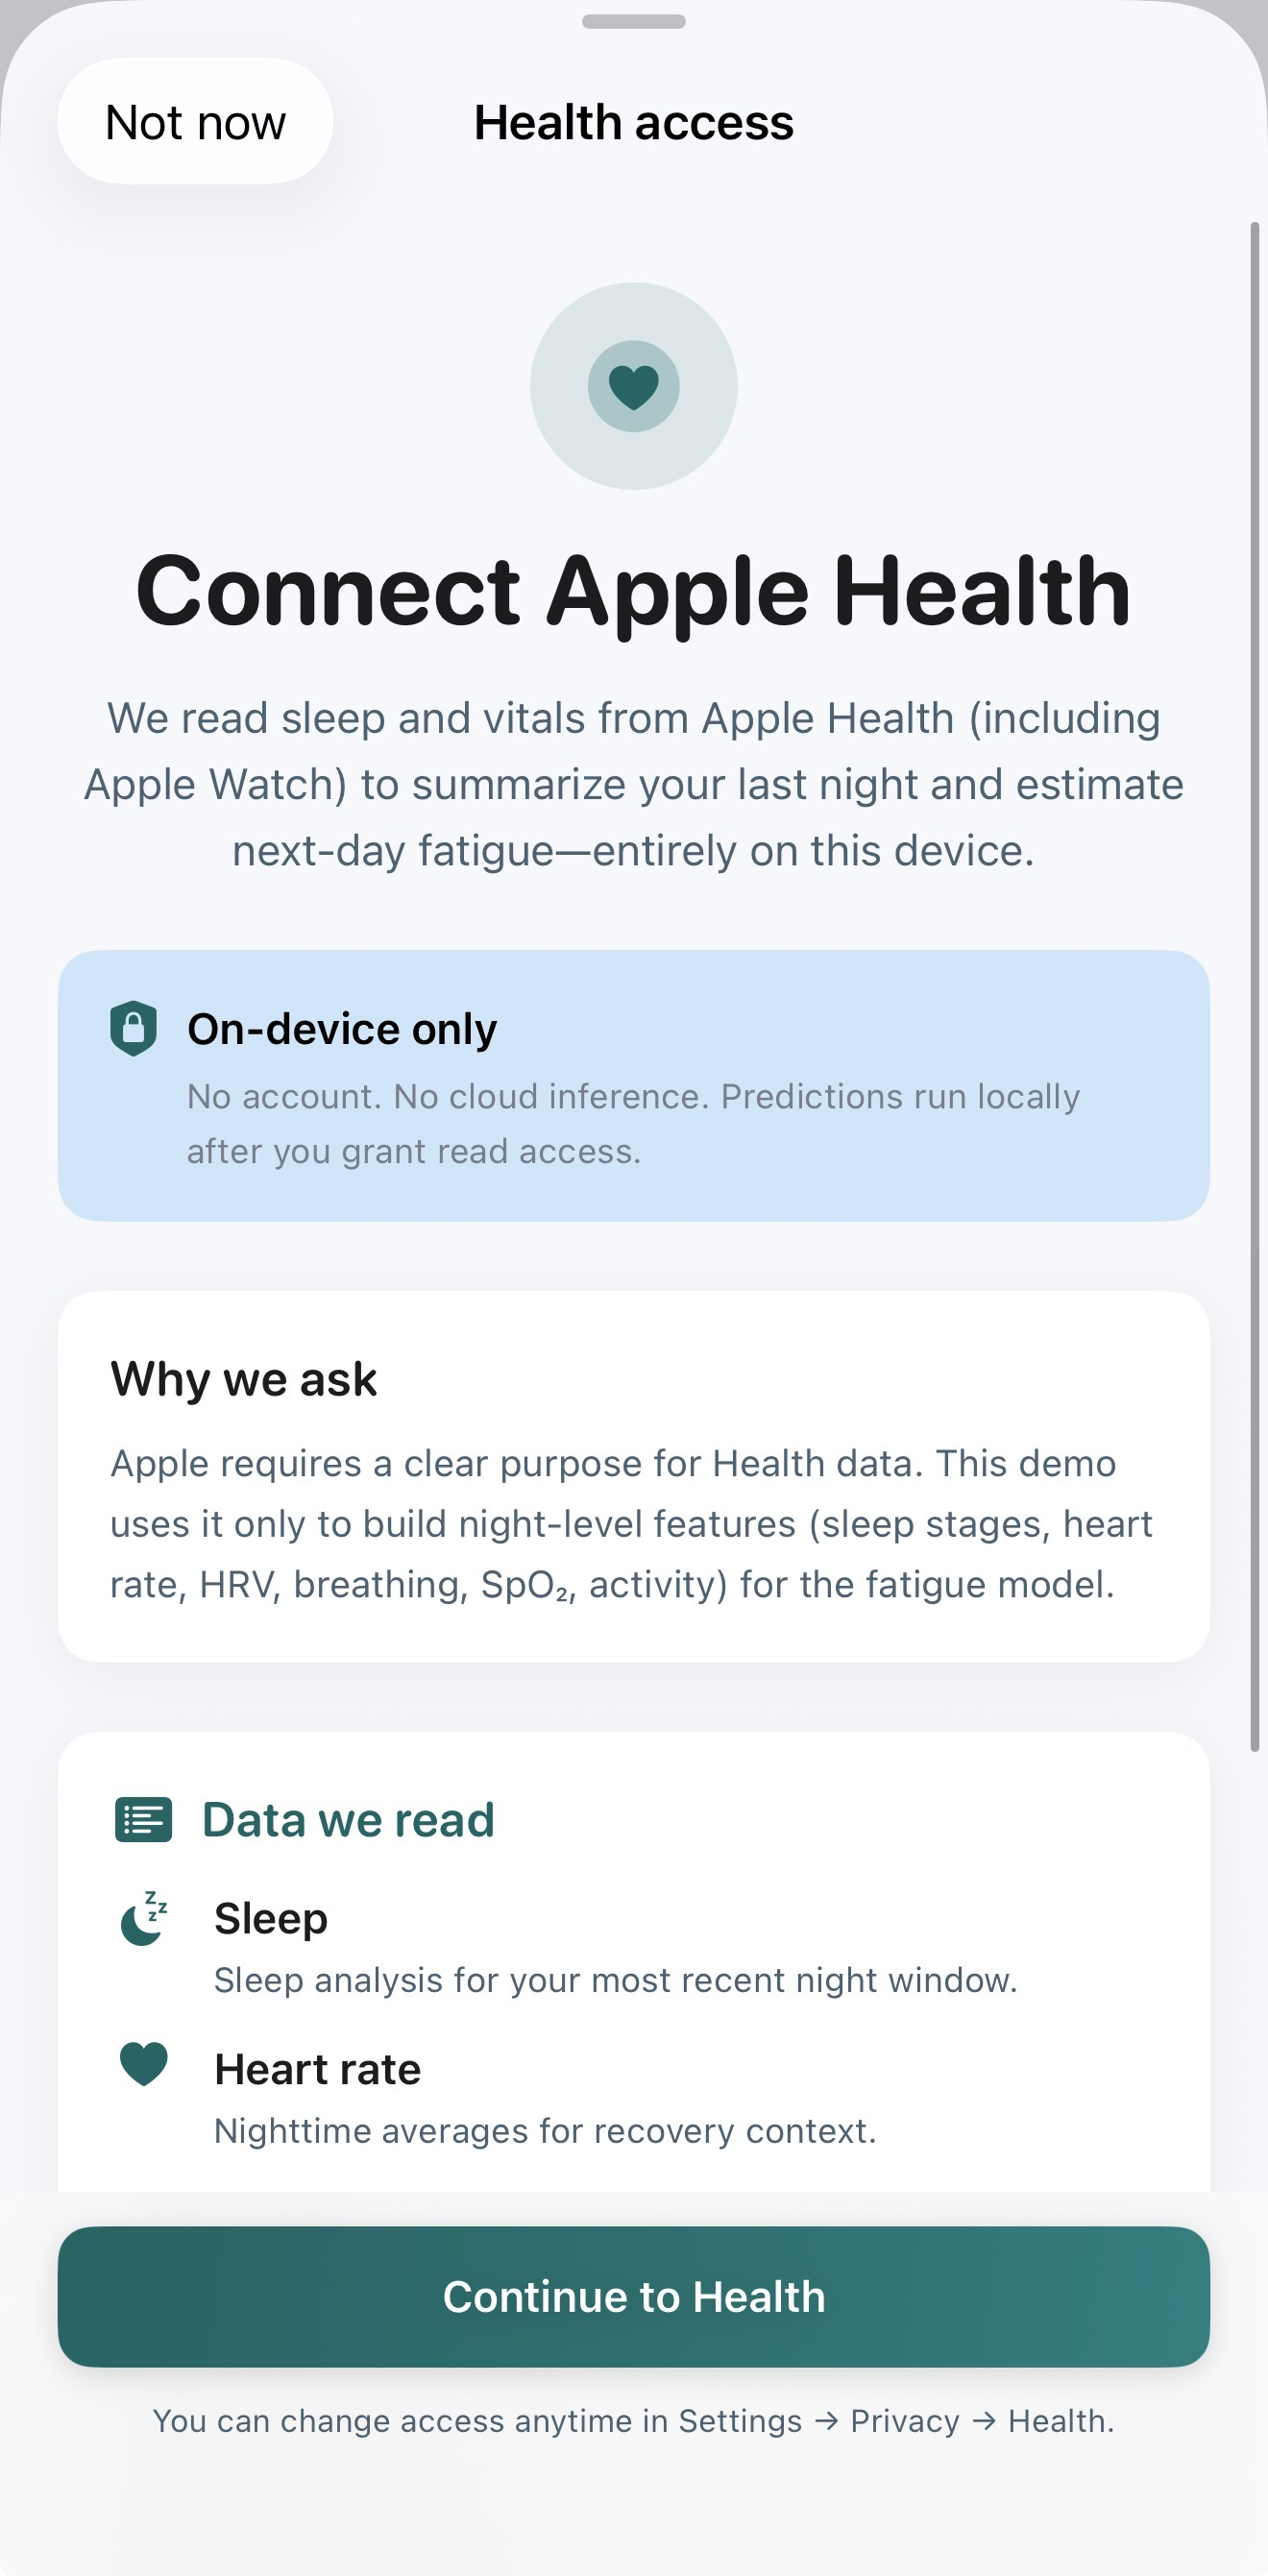
\includegraphics[width=0.24\textwidth]{IMG_4957.jpg}
  \caption{Screenshots from the system demo showing the app interface, local prediction output, and on-device history view.}
  \label{fig:demo}
\end{figure*}

The demo flow is direct. The user gives HealthKit permission, the app fetches recent Apple Watch data, the local feature builder prepares the model inputs, and the JSON contract produces the fatigue result. We used this flow because it matches the privacy goal of the project: the phone can make the prediction without sending biometric data to a server.

\section{Discussion and Limitations}

\subsection{Mobile Runtime Constraints}
The iOS prototype also showed practical runtime limits. HealthKit access requires user permission, real data is only available on a physical iPhone, and refresh behavior must respect iOS scheduling rules. For the class demo, the app uses manual fetch and prediction as the primary path, which makes the privacy behavior and data flow easier to verify.

\subsection{Addressing the Performance Ceiling}
The model performance is limited by the small and mostly single-user labeled dataset. A 52\% accuracy result should therefore be interpreted as a feasibility baseline, not as a production-quality fatigue classifier. Fatigue is subjective and can be affected by stress, workload, illness, and schedule changes that are not fully visible in sleep and vital-sign data. The main value of the project is the working mobile pipeline: data access, feature extraction, local inference, and UI feedback all run in one privacy-preserving path.

\subsection{Implementation Lessons}
The implementation clarified that a wearable ML model is only useful if the preprocessing path is reproducible on the device. The same feature names, ordering, imputation policy, and scaling parameters used during training must be available to Swift at runtime. Otherwise, the phone may compute values that look valid but no longer match the training distribution.

A second lesson is that HealthKit data is not a clean table. Samples arrive from multiple sources, some records are user-entered, and simulator data cannot replace a physical iPhone for real validation. The prototype handles this by preferring Apple Watch-origin samples when present, filtering manual entries where possible, and making missing-feature behavior explicit through the contract.

\subsection{Fixed Sleep Windows vs. Dynamic Rhythms}
A limitation of the current pipeline is the fixed night-window rule. The 6-hour shift works for a normal overnight sleep schedule, but it may fail for shift workers, naps, or irregular sleep. A better version would calculate sleep windows from the actual sleep samples instead of relying on a fixed time offset.

\subsection{Future Directions: Rolling Context}
The next step is to improve the rolling features. In particular, 3-day and 7-day HRV trends may capture recovery better than one-night summaries. More labeled users would also be needed before the model could be evaluated as a general fatigue predictor.

\section{Conclusion}

This project built and tested a mobile-first pipeline for next-day fatigue prediction from Apple Watch data. The work covered data parsing, night-window construction, feature engineering, model evaluation, JSON contract export, and Swift HealthKit integration. The model result is modest, with 52\% accuracy and 0.51 F1, so the current system should be viewed as a prototype rather than a finished fatigue classifier.

The main learning from the project is that mobile ML is not only about choosing a model. The training pipeline, feature contract, missing-value handling, HealthKit permissions, and iOS runtime constraints all have to match. Future work should focus on more labeled users, better sleep-window detection, stronger rolling recovery features, and a longer real-device evaluation.

\bibliographystyle{ACM-Reference-Format}
\bibliography{references}
\end{document}
